\documentclass[12pt]{report}
\usepackage{titlesec}

\titleformat{\subsection}[display]
{\normalfont\bfseries}{}{0pt}{\Huge}

\usepackage[a4paper]{geometry}

\usepackage{setspace}
\usepackage{graphicx}
\usepackage{natbib}
\bibliographystyle{abbrvnat}
\setcitestyle{authoryear,open={(},close={)}}
\doublespacing

\begin{document}
	\begin{titlepage}
		\centering
		\vspace*{0.5 cm}
		
\includegraphics[scale=0.75]{nust.png}	% University Logo
		\begin{center}    \textsc{\Large   NATIONAL UNIVERSITY OF SCIENCE AND TECHNOLOGY}\\[2.0 cm]	\end{center}% University Name
		\textsc{\Large 2019  }\\[0.5 cm]				% Course Code
		\rule{\linewidth}{0.2 mm} \\[0.4 cm] 
		Project Title: Sentiment Analysis for National University Of Science And Technology Library.
		\rule{\linewidth}{0.2 mm} \\[1.5 cm]
		
		
		Faculty : Applied Sciences 
		
		
		Department :Computer Science (Conv) 
		
		
		Student Name: Howard Mabhugu
		
		Student Number: N0161388M
		
		Supervisor : Mr D. Musundire
		
		
		
		\null
		This proposal document is submitted in partial fulfilment of the requirements of the BSc (Hons) Computer Science at the National University of Science  and Technology.
		
	\end{titlepage}
	
	
	\section{Project Proposal}
	\subsection{Introduction}
	Institutions are organisations that are formed for reasons that maybe religious, educational, and social. Educational libraries have an aim of improving students results in schools. Religious may have business mind and at the same time to push a certain religious belief. Social reasons have got an aim of entertaining the patrons at the same time having a business mind too. In all these library cases money is needed to finance library activities. All the libraries that are owned by institutions are departments that have their own management that is big varying from how big the library is. But all in all there is institutional management that is on top of the hierarchy where library management is supposed to report to.  The bigger the library is, the more staff it requires and the more its day to day activities goes unnoticed by the institutional management. The more the patrons that are served at the library the more difficulty it is for the institutional management to receive feedback about the services being delivered in the library straight from the patrons. If there is little to non-feedback about the services that are being offered in the library the more vulnerable the library patrons are to poor service delivery.\\
	
	Patrons have different experiences and expectations in any organisation they are attached to (Hogg and Hogg, 1995;Perez, Juan, Gema and  Raquel,2007),for instance, patrons wants quality and enough information, their expectations for better service performance is increasing, therefore increased patron satisfaction is important(Doherty, 1994;Rasli,Danjuma, Yew \& Igbal,2011). Patron satisfaction must be a key goal of every institution or organisation as it builds patron loyalty and goodwill of the organisation. Patron satisfaction can be increased by interacting with them. Interacting with the patrons means the libraries give them a platform where they can give feedback (positive or negative) about the services they are receiving in the library. If top institutional management interacts with patrons they feel included in the activities of the library, they feel appreciated and they feel belonging to the library. If they feel belonging to a library, they become loyal to it thereby building good patron base. The platform that will be used must be effective so as to motivate the patrons to give more feedback in the future. If patrons complain are being respondent to, then they get motivated to leave feedback after receiving a service. This project is going to provide a better platform for library patrons to leave their feedback and it will produce reports for the top institutional management about the service delivery in the library. The project will allow patrons to interact with the management not only in cases where service delivery has deteriorated but also in times of good service delivery. The more the institutional management interact with the patrons, the more they discover problems while they are still emanating, other than when they are at manifestation stages. The earlier problems are discovered the lesser complicated they are, the easier they are to solve.
	
	\subsection{Background}
	Institutional libraries are mainly for educational institutions in Zimbabwe, though some religious institutions own libraries as well. The reasons for owning these libraries varies from institution to institution but all in all there is need for funds and there is need for patron satisfaction. In order to satisfy patrons library management must allow patrons to give feedback about services they are receiving. In return to the effort of patrons, management must respond to all the positive feedback through correcting the faults. The interaction between patrons and management is something that can’t be underrated as far as better delivery and goodwill of the library is concerned see \citep{esuli2006sentiwordnet}. The interaction between customers and any organisation offering a service is something that people normally do when there is poor service delivery. The energy to give the feedback been driven by anxiety. To get a full understanding of how people underrate customer interaction see \cite{PINE}.\\ 
	Patrons are currently using online methods (email, WhatsApp), offline methods (suggestion box) and calls \citep{pasquale2011system} to launch their feedback. The institutional management has to take a thorough reading of the feedback returned by patrons and derive a conclusion of service delivery from the information left by patrons. This isn’t a problem if an institution is small, the feedback they receive s all small. The problem comes to larger institutions where there is probability of getting thousands of feedback about service delivery in a week, especially if there is poor service delivery. It won’t be economic in terms of time to go through all the messages. \\	
	A lot of institutions invested a lot into sentiment analysis systems. According to research by \cite{gamon2004sentiment} on a number of sentient analysis systems that where done for different organisations there is one problem that is coming up. The problem is difficulty to perform sentiment analysis on noisy patron feedback. Noisy feedback is a feedback that has got contents that does not tally up or make sense even to a human being as far as the topic or issue of discussion is concerned. Analysis of noisy data/feedback will never bring anything useful in hand, thereby it justifies omitting of feedback that contains such data during analysis and report generation.\\
	Valuing the effort that patrons put when it comes to giving feedbacks is something that every institution must do and in return take action for all the positive feedbacks that patrons pass.
	
	
	\subsection{Problem Statement}
There is no platform that captures patron feedback and analyse it efficiently for institutional management. Due to the number of patrons that belong to institutional libraries in Zimbabwe, it is difficult for management to personally view every feedback left by patrons using the current methods of leaving feedbacks. This brings a big problem where positive feedback left by patrons is not viewed always. 
	\subsection{Aim}
	To develop a web based system for analysing patrons feedback and generate report for library service delivery at a particular period of time.
	\subsection{Objectives}
	\begin{enumerate}
		\item To allow patrons to leave feedback on the website anonymously.
		\item To generate periodic reports.
		\item  To omit noisy feedback / data during analysis.
	\end{enumerate}
	
	
	\subsection{Justification}
	The system will help in a lot of ways to institutional libraries. This includes allowing patrons to leave feedback about service delivery anonymously, alerting for poor library service delivery at early stages and the system will reduce task overload on top management.\\
	The system will allow patrons to leave feedback in the system anonymously. That means they won’t be afraid to express their feelings or mentioning names of staff delivering poor services since their personal details will be hidden. No one will know who left a comment in the system.\\
	In addition, the system will also help the institution management by alerting for upcoming of a problem in the library early. The earlier a problem is discovered the easier it is to find the cause and fix it thereby maintaining library goodwill. The system will accomplish this by producing reports about library performance.\\
	\\Moreover, the system will reduce poor service delivery within institutional libraries. The top institution management won’t be in the field with patrons and the system will provide reports of the activities that are done in the libraries basing from customer feedback. The fact that patrons will be giving feedback to the institution this piles pressure on the library staff to deliver quality and satisfactory services to the patrons.\\
	Sentiment analysis saves management time of going through each and every comment that patrons leave one by one. The system will analyse the comments and produce a report that summarise the comments from patrons instead of management analysing the comments on their own.
	
	\subsection{Methodology}
	In this project I am going to adopt the use of supervised feature selection project management methodology. Feature selection is actually a process whereby irrelevant or unneeded elements are removed and the only needed elements are kept. So supervised feature selection methodology removes unnecessary data elements and remain with few important data elements. This methodology is best fit for my project as it helps to by cleaning the datasets so that necessary data remains. Not every feature in a data set is required at every stage. Some of the features will be best if neglected. That will make feature selection suitable in this project.
	
	\subsection{Scope}
	The project will focus on the development of a sentiment analysing system for educational institutions that is universities in specific and generate reports for top institutional management.
	\subsection{Expected Outcome}
	Once everything is done, the project is supposed to produce a system that will be able to let users leave feedback on the website about library services after getting a service from the library anonymously. This kills fear from the patrons as they know that they won’t be exposed.\\
	The system will generate reports for the institution management. The reports will be scheduled reports or as per management request. All these will improve service delivery within institutional libraries at the same time satisfying patrons as far as service delivery is concerned.\\
	Moreover, management may also have need for reports for a specific period of time, so the system must be able to provide this service. If management request a report from 1 January 2019 to 29 June 2019 the system must be able to analyse customer comments and produce a report for that period.\\
	
	Lastly the system must omit noisy data/ feedback. Noisy data is nonsensical data that if even combined or interpreted won’t produce any useful information. Analysis of that data will be just wasting of time so omitting it will be the best thing.
	
	\subsection{Project Schedules}
	
	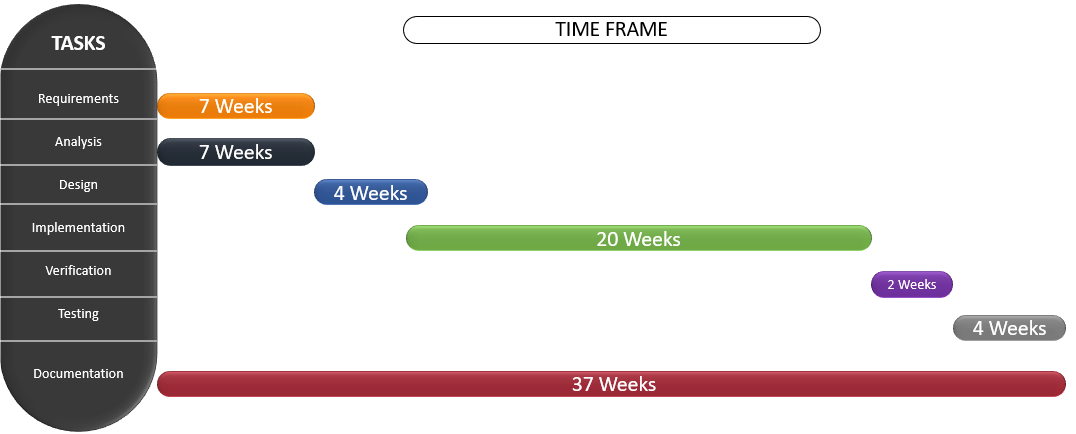
\includegraphics[scale=0.5]{gant.png}
	
	\section{Literature Review}
	\subsection{Introduction}
	Sentiment analysis is a field that allows interaction between human beings and computers using natural language. This field allows listening to the Voice of Customers. It is being applied in different fields like politics, marketing and also learning. Sentiment analysis is the process of analysing opinions expressed in form of text computationally with normally a goal of obtaining the attitude of someone towards a certain topic / subject. This chapter describes sentiment analysis and the fields that are currently using it, effort that was directed towards using it and technologies that are currently being used to cater for Voice of Customers in businesses.
	
	\subsection{Sentiment Analysis Definitions}
	Different and multiple efforts where put in place with the aim of giving the best definition that brings out all the elements covered by sentiment analysis in a single line. The term itself has got different names that are used to means the same with it that suit best with the subject of application at a particular period of time. Authors are using the different names in accordance to the subject. It is sometimes called opinion mining \citep{pang2008opinion} and also polarity detection \citep{sharma2014polarity}.   \\
	 \cite{esuli2006sentiwordnet} defined opinion mining/sentiment analysis as a recent discipline at the crossroads of information retrieval and computational linguistics which is concerned not with the topic a document is about, but with the opinion it expresses. This definition is far much too broad and it put focus on document level sentiment analysis. Document level sentiment analysis is normally not appropriate as it take the whole document as a single entity. Therefore the definition is not specific enough to define sentiment/ opinion mining in library terms. \\
	\citep{priyasentiment} defined “Sentiment analysis is the process of analysing the affective text into positive ,negative or neutral emotions.” This definition misses out the techniques that are used that is Natural Language Processing, computational analysis and linguistical and textual analysis. Adding the techniques to the definition, a new definition which states that Sentiment analysis is a data mining type that looks for inclination from people’s opinions using natural language processing, text analysis and computational linguistics, which their use is to extract and analyse subject related information from different sources. This definition suits best sentiment analysis for a library system.\\
	\subsection{Existing Technologies Of Capturing Voice Of Customers
		
	\bibliography{refs}
\end{document}
